\documentclass{article}

\usepackage{microtype}
\usepackage{graphicx}
\usepackage{booktabs}
\usepackage{hyperref}

% Default to the anonymous review format.
% Switch to \usepackage[accepted]{icml2026} for the camera-ready version.
\usepackage{icml2026}

\usepackage{amsmath,amssymb,amsthm,mathtools}
\usepackage{enumitem}
\usepackage[capitalize,noabbrev]{cleveref}

\theoremstyle{plain}
\newtheorem{theorem}{Theorem}[section]

\newcommand{\HM}{\mathrm{HM}}
\newcommand{\AM}{\mathrm{AM}}
\newcommand{\Var}{\mathrm{Var}}
\newcommand{\E}{\mathbb{E}}
\newcommand{\proj}{\operatorname{proj}}
\newcommand{\placeholderfigure}[3]{
  \begin{figure}[t]
  \centering
  \fbox{
    \begin{minipage}{0.94\linewidth}
    \small
    \textbf{#1}
\par\vspace{0.5em}
    #2
    \end{minipage}
  }
  \caption{#3}
  \end{figure}
}

\icmltitlerunning{Evidence-Weighted and Opponent-Shaped Policy Gradient}

\begin{document}

\twocolumn[
\icmltitle{Evidence-Weighted and Opponent-Shaped Policy Gradient with Composed Convergence Guarantees}

\begin{icmlauthorlist}
\icmlauthor{Anonymous Author}{anon}
\end{icmlauthorlist}

\icmlaffiliation{anon}{Anonymous Institution}
\icmlcorrespondingauthor{Anonymous Author}{anonymous@icml.cc}
\icmlkeywords{multi-agent reinforcement learning, policy gradient, stochastic games}

\vskip 0.3in
]

\printAffiliationsAndNotice{}

\begin{abstract}
Policy-gradient methods in general stochastic games now admit local convergence guarantees to stable Nash policies, but two practical weaknesses remain. First, agents often learn from observations of uneven quality, so equal-weight updates let the noisiest gradients dominate the joint dynamics. Second, even when a stable Nash policy exists, the basin of attraction may be small, making convergence sensitive to initialisation. We study two modifications that address these weaknesses without leaving the convergence regime of \citet{giannou2022convergence}. Evidence-weighted policy gradient (EW-PG) rescales each agent's update by an inverse-variance evidence weight and reduces the effective gradient variance by a factor $\HM(V)/\AM(V)\leq 1$. Opponent-shaped policy gradient (LOLA-PG) adds a one-step opponent-shaping term and, under an annealed shaping schedule, preserves local convergence while enlarging the stable basin when the shaping Hessian satisfies a spectral reinforcement condition. Our main contribution is a composition theorem: under the union of the EW and LOLA assumptions, EW-LOLA-PG inherits both the variance reduction and the basin enlargement. The draft is supported by completed matrix-game, basin-mapping, and persona-conditioned iterated-game runs, with explicit placeholder slots reserved only for the remaining workshop figures.
\end{abstract}

\section{Introduction}

Policy-gradient learning in multi-agent systems long lacked trajectory-level convergence guarantees outside narrow game classes. \citet{giannou2022convergence} changed that picture by proving local convergence to stable Nash policies in general stochastic games under a stable second-order condition. That theorem gives a clean baseline, but it does not by itself solve two problems that matter in practice. The first is heteroskedasticity across agents: gradient estimators can have sharply different variances because agents observe different histories and occupy different informational positions in the game. The second is geometric: local convergence only helps when initialisation lands in the attraction region of the target equilibrium, and that region may be small.

This paper studies two modifications that target those problems on orthogonal axes. Evidence-weighted policy gradient (EW-PG) scales each agent's update by a Keynesian evidence weight proportional to the inverse of its gradient variance. In the Omega technical report, this yields a simple harmonic-mean versus arithmetic-mean variance improvement while preserving the Giannou convergence rate constant up to the same factor \citep{shcherbinin2026omega}. Learning with Opponent-Learning Awareness (LOLA) takes a different route. \citet{foerster2018lola} introduced a shaping term that anticipates how the current agent changes the opponent's next update. The original paper showed strong behavioural effects in iterated prisoner's dilemma and convergence to Nash play in repeated matching pennies, but it did not provide a general local convergence theorem for stochastic games. The Omega report adds that missing layer by annealing the shaping schedule and proving both rate preservation and, under a spectral reinforcement condition, an enlarged stable basin \citep{shcherbinin2026omega}.

The main claim of this paper is that these two improvements compose cleanly, but that conclusion is not automatic. Evidence weights multiply the same coordinates that LOLA shapes, so they could in principle damp the shaping benefit, distort the favourable Jacobian symmetry, or couple online weight-estimation noise to the shaping bias. The composition result matters because the local Lyapunov recursion separates these effects: evidence weighting changes the martingale variance constant, whereas annealed LOLA changes the bias budget and the local drift. Under a weighted spectral condition on the shaped Jacobian, no additional mixed term is needed. The resulting algorithm, EW-LOLA-PG, is a workshop-sized distillation of the broader Omega-gradient programme.

We make four contributions. First, we restate the \citet{giannou2022convergence} setup in the minimal form needed for a workshop audience. Second, we isolate the EW-PG result as a variance-reduction theorem with preserved local convergence. Third, we isolate the LOLA-PG result as a rate-preserving opponent-shaping method with a basin-enlargement theorem. Fourth, we state a composition theorem showing that EW-LOLA-PG inherits both improvements under the union of the separate assumptions.

\section{Preliminaries}

We work with finite stochastic games in the tabular episodic setting. A game is given by
\begin{equation}
G = (N,S,\{A_i\}_{i\in N},\{R_i\}_{i\in N},P,\rho),
\end{equation}
where $N$ is the set of agents, $S$ is the state space, $A_i$ is agent $i$'s action set, $R_i$ is its reward function, $P$ is the transition kernel, and $\rho$ is the initial-state distribution. Each agent chooses a stationary Markov policy $\pi_i \in \Pi_i = \Delta(A_i)^{|S|}$, and the joint policy space is $\Pi=\prod_i \Pi_i$.

For each agent $i$, let $V_{i,\rho}(\pi)$ denote the expected episodic return under joint policy $\pi$, and let
\begin{equation}
v_i(\pi)=\nabla_{\pi_i}V_{i,\rho}(\pi)
\end{equation}
be the policy gradient. Writing $v(\pi)=(v_i(\pi))_{i\in N}$, the projected policy-gradient update takes the form
\begin{equation}
\pi_{n+1}=\proj_{\Pi}(\pi_n+\gamma_n \hat v_n),
\end{equation}
where $\hat v_n$ is a stochastic gradient estimator, such as REINFORCE, and $\gamma_n=\gamma/(n+m)^p$.

The relevant equilibrium notion is the stable Nash policy from \citet{giannou2022convergence}. We use the second-order stationary refinement because it yields a quantitative drift inequality. A Nash policy $\pi^\ast$ satisfies the local stability condition if there exists $\mu>0$ such that, for all $\pi$ in a neighbourhood of $\pi^\ast$,
\begin{equation}
\langle v(\pi), \pi-\pi^\ast \rangle \leq -\mu \|\pi-\pi^\ast\|^2.
\end{equation}
Under the regularity assumptions in \citet{giannou2022convergence}, if the initial policy lies in the relevant neighbourhood and the stochastic bias and variance exponents satisfy the usual stochastic-approximation conditions, then projected policy gradient converges to $\pi^\ast$ with
\begin{equation}
\E[\|\pi_n-\pi^\ast\|^2\mid E] = O(C / n^q),
\end{equation}
for an event $E$ of high probability and exponent $q=\min(\ell_b,p-2\ell_\sigma)$.

We only need three ingredients from that framework: a local drift inequality near the target Nash policy, a bias bound for the gradient estimator compatible with the step-size schedule, and a variance bound that lets the martingale term be controlled at rate $O(n^{-q})$. Everything below is built to preserve those ingredients while improving either variance or basin geometry.

\section{Evidence-Weighted Policy Gradient}

\subsection{Setup}

In multi-agent learning the agents do not observe the game through equally informative histories. Some sit in stable information states with low-variance gradient estimates; others face noisier observations or more weakly identified best responses. Standard joint policy gradient ignores that heterogeneity. Every agent receives the same global step-size even when its estimator is much noisier than the rest.

Let $V_{i,n} = \Var(\hat v_{i,n})$ denote the variance of agent $i$'s gradient estimator at iteration $n$, and define
\begin{equation}
w_{i,n}=\frac{V_{\min,n}}{V_{i,n}},
\qquad
V_{\min,n}=\min_j V_{j,n}.
\end{equation}
Agents with the lowest variance receive weight $1$, and noisier agents are downweighted proportionally. The EW-PG update is
\begin{equation}
\pi_{i,n+1}=\proj_{\Pi}(\pi_{i,n}+\gamma_n w_{i,n}\hat v_{i,n}).
\end{equation}

The convergence theorem below is stated for oracle or frozen local variances because that is the clean stochastic-approximation setting. In practice, the weights must be estimated from rollouts. A natural plug-in estimator uses a running window of recent gradients
\begin{equation}
\begin{aligned}
\hat \sigma^2_{i,n}
&=
\frac{1}{M-1}\sum_{k=n-M+1}^{n}
\left\lVert g_{i,k}-\bar g_{i,n}\right\rVert^2,\\
\hat w_{i,n}
&=
\frac{1/\hat \sigma^2_{i,n}}{\max_j 1/\hat \sigma^2_{j,n}}.
\end{aligned}
\end{equation}
which is consistent under local stationarity of the gradient process over the window \citep{shcherbinin2026diss}. The resulting plug-in weights converge to the oracle weights as the window fills, but they also introduce an additional transient estimation error. We therefore distinguish sharply between the oracle theorem and the practical estimator. The current experiments still use oracle weights, and an online-weight ablation remains required before submission.

\subsection{Variance Improvement and Convergence}

\begin{theorem}[AM-HM variance improvement]
Let $V_i=\Var(\hat v_i)$ denote the per-agent gradient variances. Under EW-PG, the effective variance of the joint update satisfies
\begin{equation}
\sigma_w^2
=\frac{\HM(V)}{\AM(V)}\sigma_{\mathrm{std}}^2
\leq \sigma_{\mathrm{std}}^2,
\end{equation}
with equality if and only if all $V_i$ are equal.
\end{theorem}

\noindent\textbf{Proof sketch.} The weighted variance sum is $\sum_i w_i^2 \sigma_i^2$. Substituting $w_i=V_{\min}/V_i$ and $\sigma_i^2\propto V_i$ yields the harmonic-mean normalisation. The inequality is exactly the AM-HM inequality.

\begin{theorem}[Convergence of EW-PG with oracle weights]
Under the hypotheses of \citet[Theorem 1]{giannou2022convergence}, and with exact or locally frozen variance weights, EW-PG converges to a stable Nash policy with
\begin{equation}
\E[\|\pi_n-\pi^\ast\|^2\mid E]
= O\!\left(\frac{\HM(V)}{\AM(V)}\cdot \frac{C}{n^q}\right).
\end{equation}
\end{theorem}

The rate exponent stays the same. The gain appears in the leading constant, which shrinks by the harmonic-to-arithmetic mean ratio. The local convergence machinery remains intact.

EW is best viewed as a residual step-allocation rule, not as a replacement for standard variance-reduction tools. Counterfactual baselines and centralised critics such as COMA reduce the variance of each agent's own policy-gradient estimator by using richer conditioning information \citep{foerster2018coma}. Optimal-baseline analyses for multi-agent policy gradients play a similar role \citep{kuba2022variance}. EW addresses a different question: once residual estimator variances remain heterogeneous across agents, how should a shared joint update allocate trust across them? Increasing rollout counts can also equalise variances, but that raises sample cost and may be infeasible when agents have asymmetric observation channels or fixed interaction budgets. For that reason, EW is orthogonal to critics, baselines, and larger batch sizes rather than a substitute for them.

\section{Opponent-Shaping Policy Gradient}

\subsection{The LOLA Correction}

\citet{foerster2018lola} introduced Learning with Opponent-Learning Awareness as a way to account for the fact that the current agent changes the opponent's next update. In its simplest form, the method augments the policy gradient with a one-step opponent-shaping term,
\begin{equation}
\mathrm{OS}_i(\pi)
= \sum_{j\neq i}\frac{\partial R_i}{\partial \theta_j'}\frac{\partial \theta_j'}{\partial \theta_i},
\end{equation}
where $\theta_j' = \theta_j - \eta_j \nabla_{\theta_j}R_j$ is agent $j$'s anticipated one-step update.

The technical report closes the theory gap by using an annealed shaping coefficient
\begin{equation}
\lambda_n = \lambda/(n+m)^r,
\end{equation}
with $r>1-p$. The resulting update is
\begin{equation}
\pi_{i,n+1}
= \proj_{\Pi}\bigl(\pi_{i,n}+\gamma_n(\hat v_{i,n}+\lambda_n \mathrm{OS}_{i,n})\bigr).
\end{equation}

The theorem in this section is explicitly about the Jacobian of the one-step field $\mathrm{OS}(\pi)$ defined above. It does not claim that one-step opponent modelling captures every relevant adaptation effect. Multi-step meta-gradients such as Meta-MAPG differentiate through longer update chains and therefore study a richer object \citep{kim2021meta}. The claim here is narrower: the one-step LOLA field already has a local Jacobian whose symmetric part can improve contraction near a stable Nash point.

\subsection{Convergence and Basin Enlargement}

\begin{theorem}[Annealed LOLA preserves convergence]
Suppose the baseline policy-gradient assumptions of \citet{giannou2022convergence} hold, and let $\lambda_n=\lambda/(n+m)^r$ with $r>1-p$. Then LOLA-PG converges to the same stable Nash policy at the same rate exponent $q$ as standard policy gradient.
\end{theorem}

\noindent\textbf{Proof sketch.} The opponent-shaping term contributes an additional bias of order $O(\lambda_n G)$, where $G$ bounds the local shaping correction. Because $\lambda_n$ decays faster than the threshold implied by $p+\min(\ell_b,r)>1$, the aggregated bias still satisfies the summability condition needed in the martingale argument.

Let $H=\nabla_\pi \mathrm{OS}(\pi^\ast)$ denote the Jacobian of the opponent-shaping field at the target equilibrium, and let $S_H=(H+H^\top)/2$ be its symmetric part.

\begin{theorem}[Basin enlargement under spectral reinforcement]
If $S_H$ is negative semidefinite with largest eigenvalue $-\mu_H$ for $\mu_H\geq 0$, then LOLA-PG improves the local drift parameter from $\mu$ to
\begin{equation}
\mu_{\mathrm{LOLA}}=\mu+\lambda \mu_H > \mu.
\end{equation}
\end{theorem}

The conclusion is local but meaningful. A larger drift constant means a stronger inward pull around the stable Nash point, which translates into a larger attraction region and faster contraction inside that region.

The spectral reinforcement condition is restrictive, but it is not opaque. The extended dissertation gives two sufficient cases that match the usual intuition for LOLA-style methods \citep{shcherbinin2026diss}. First, in two-player zero-sum games the base gradient field typically has a strong antisymmetric, rotational component, and opponent shaping converts part of that rotation into contraction. Second, locally negative cross-Hessians also favour reinforcement because the agents' objectives pull against one another in a way that the shaping term can stabilise. By contrast, potential games need not benefit: if the base field is already locally contractive and mostly symmetric, there may be little rotational structure for LOLA to exploit. This domain dependence is why the present theorem is aimed at competitive games such as matching pennies or rock-paper-scissors, not at every iterated game used elsewhere in the empirical section.

The practical meaning of $\mu_{\mathrm{LOLA}}>\mu$ should also be stated carefully. Theorem 4.2 does not yield a global closed-form volume for the attraction basin. Its content is local: if higher-order remainder terms are bounded in a neighbourhood of $\pi^\ast$, then a larger drift margin lets the same Lyapunov argument absorb those remainders on a weakly larger neighbourhood. The empirical question is therefore initialisation sensitivity near equilibrium, not a global measure of basin size.

\section{Composition: EW-LOLA-PG}

We combine the two modifications. Let $W_n=\mathrm{diag}(w_{1,n},\ldots,w_{N,n})$ denote the local evidence-weight matrix, and suppose that on the neighbourhood where the theorem is applied the weights remain bounded away from zero and converge to a local limit $W^\ast$.
\begin{equation}
\pi_{i,n+1}
=\proj_{\Pi}\bigl(\pi_{i,n}+\gamma_n w_{i,n}(\hat v_{i,n}+\lambda_n \mathrm{OS}_{i,n})\bigr).
\end{equation}

\begin{theorem}[EW-LOLA composition]
Assume the local regularity, step-size, bias, and variance conditions of \citet{giannou2022convergence}, the evidence-weight assumptions used for EW-PG, the annealed shaping schedule $\lambda_n=\lambda/(n+m)^r$ with $r>1-p$, and a local weight limit $W^\ast$. Let $\mu_W$ denote the drift constant of the weighted baseline field $W^\ast v(\pi)$, and let
\begin{equation}
H_W = W^\ast H,
\qquad
S_{H,W} = \frac{H_W + H_W^\top}{2}.
\end{equation}
If $S_{H,W}$ is negative semidefinite with largest eigenvalue $-\tilde\mu_H$ for $\tilde\mu_H\geq 0$, then EW-LOLA-PG converges locally to the same stable Nash policy with
\begin{equation}
\E[\|\pi_n-\pi^\ast\|^2\mid E]
=O\!\left(\frac{\HM(V)}{\AM(V)}\cdot \frac{C}{n^q}\right),
\end{equation}
and local drift parameter
\begin{equation}
\mu_{\mathrm{EW-LOLA}} = \mu_W + \lambda \tilde\mu_H.
\end{equation}
In particular, the algorithm inherits the EW variance reduction and preserves the LOLA drift gain whenever the weighted spectral condition holds.
\end{theorem}

\noindent\textbf{Proof sketch.} The non-trivial issue is exactly the one a skeptical reader should worry about: the evidence weights multiply the shaping term as well as the noisy gradient, so weighting could in principle preserve the variance benefit while killing the geometric benefit. The theorem rules that out only under a weighted spectral condition on $S_{H,W}$, not unconditionally. With that caveat in place, the Lyapunov recursion remains modular. Evidence weighting changes the variance term, annealed opponent shaping changes the bias term, and the weighted Jacobian controls the local drift. No new mixed term appears because the recursion already separates bias and martingale variance additively in the local analysis \citep{shcherbinin2026diss}. In the special case $W^\ast=cI$, the theorem reduces to a common scalar rescaling of both the baseline drift and the shaping gain.

The paper is intentionally narrow. \citet{giannou2022convergence} provide the convergence baseline. The dissertation supplies the measure-theoretic and stochastic-approximation scaffolding behind that baseline \citep{shcherbinin2026diss}. The Omega technical report isolates the separate EW and LOLA improvements \citep{shcherbinin2026omega}. The new step in this paper is the explicit composition theorem together with a workshop-sized empirical suite focused on that theorem.

\section{Empirical Validation}

The experiment section should stay tightly matched to the theorem structure. Four experiments are enough for the workshop version.

\subsection{Variance Reduction in Matrix Games}

This experiment validates the EW variance theorem. We compare standard PG, EW-PG, LOLA-PG, and EW-LOLA-PG on matching pennies and rock-paper-scissors under controlled noise heterogeneity.

\begin{figure}[t]
\centering
\IfFileExists{experiments/artifacts/medium_matrix/matrix_summary.png}{
  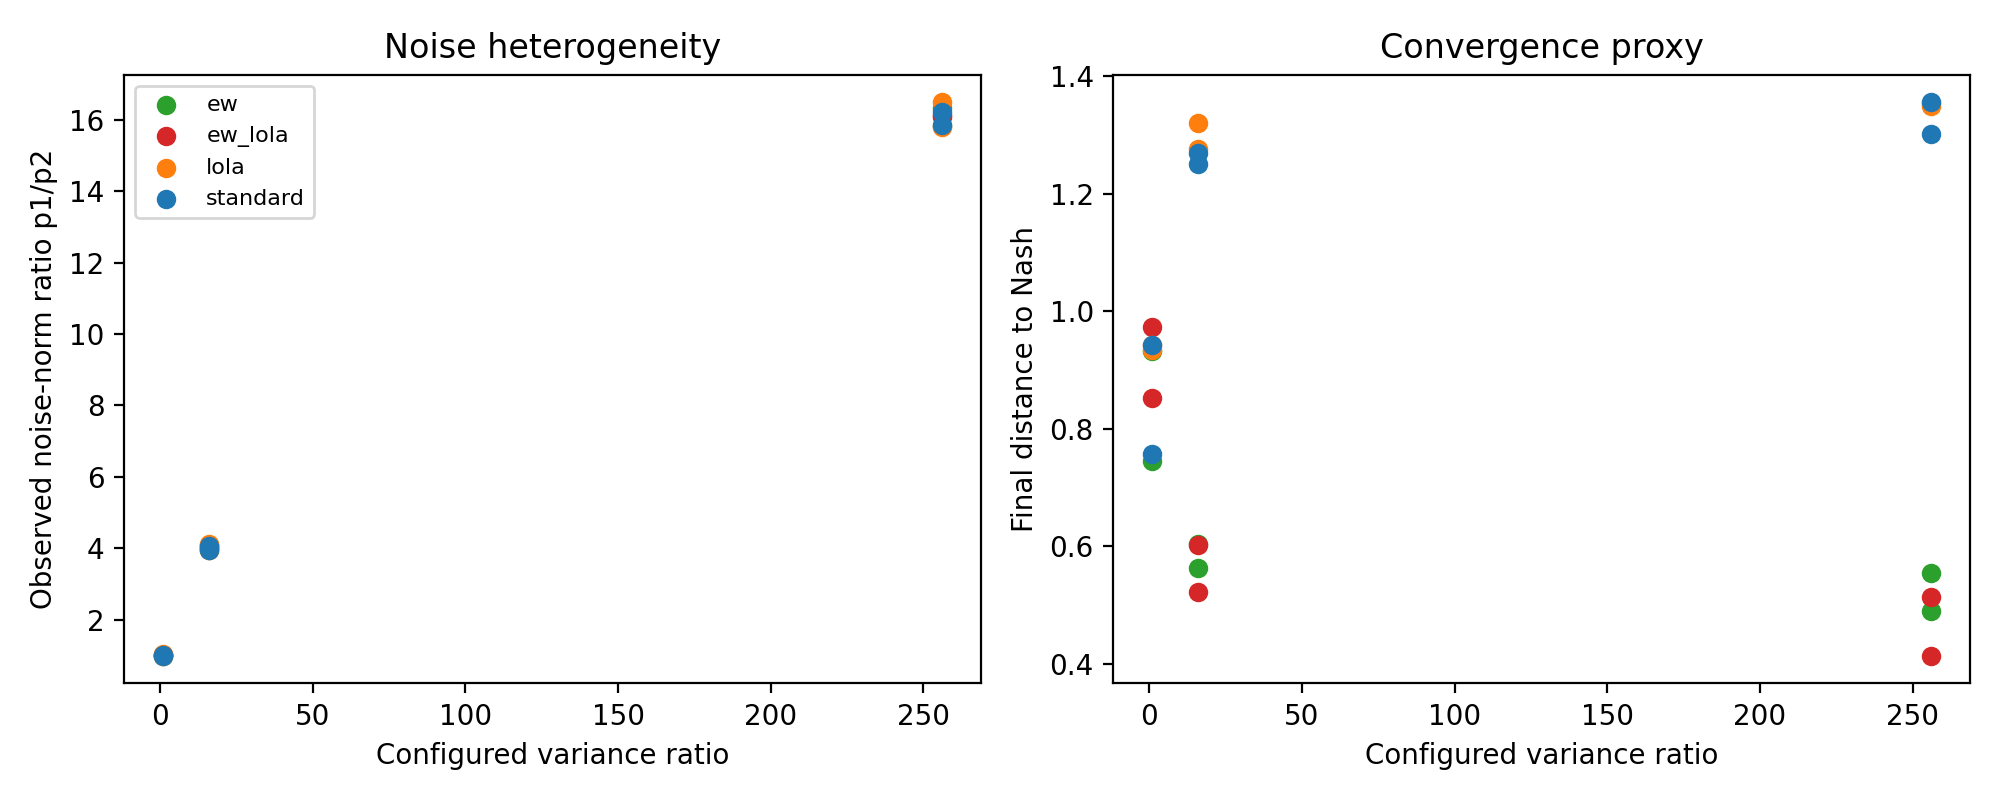
\includegraphics[width=\linewidth]{experiments/artifacts/medium_matrix/matrix_summary.png}
}{
  \fbox{\begin{minipage}{0.94\linewidth}\small
  \textbf{Figure 2 placeholder.}

  Matrix-game variance and convergence proxy. Left: noise heterogeneity versus observed variance proxy under \texttt{standard}, \texttt{ew}, \texttt{lola}, and \texttt{ew\_lola}. Right: final distance-to-Nash proxy versus heterogeneity level.
  \end{minipage}}
}
\caption{Current exploratory matrix-game output. The completed medium sweep already shows that under asymmetric noise, EW-LOLA combines the stability gains of evidence weighting with the shaping gains of LOLA. The final submission should replace this exploratory figure with a paper-ready version built from the same artifact family.}
\label{fig:matrix}
\end{figure}

The current completed sweep is saved in the repository artifacts. In the present scaffold, EW-LOLA is best under heterogeneous noise on both matching pennies and rock-paper-scissors, while pure LOLA degrades sharply in the most asymmetric settings. These runs validate the oracle AM-HM story, not the online estimator story; the latter still needs a separate plug-in-weight ablation.

\subsection{Basin Enlargement in Iterated Prisoner's Dilemma}

This experiment is the key empirical test for Theorem 4.2. We therefore use a theorem-facing setup: deterministic matching-pennies dynamics, symmetric logit initialisations around the mixed Nash point, and constant $\lambda$ so that the geometric effect is visible without annealing it away. The relevant quantity is local initialisation sensitivity near the target Nash point, not a global notion of basin volume.

\begin{figure}[t]
\centering
\IfFileExists{experiments/artifacts/basin_matrix/basin_map.png}{
  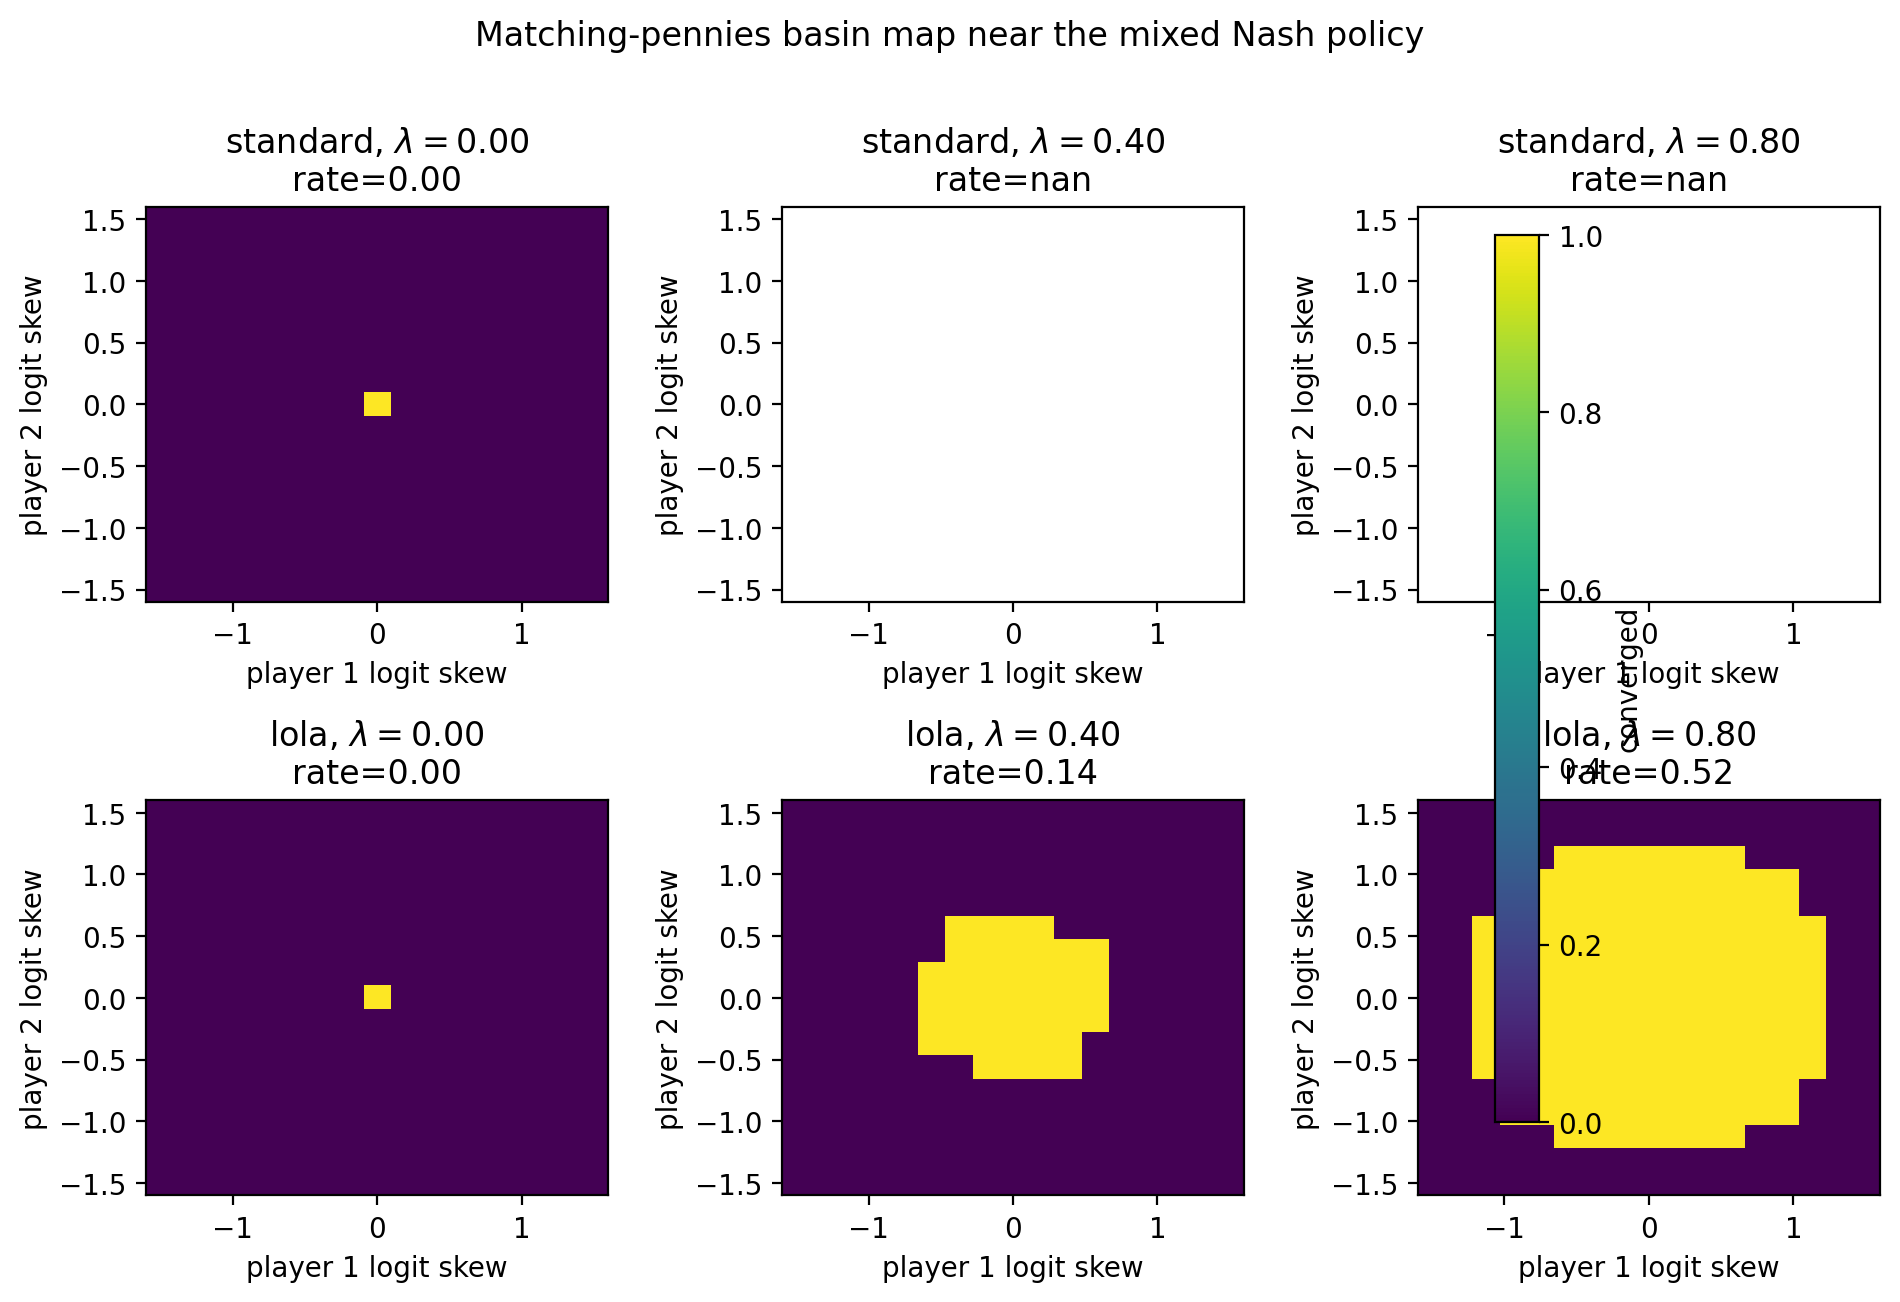
\includegraphics[width=\linewidth]{experiments/artifacts/basin_matrix/basin_map.png}
}{
  \fbox{\begin{minipage}{0.94\linewidth}\small
  \textbf{Figure 3 placeholder.}

  Matching-pennies basin map over symmetric logit initialisations. Standard PG converges only in a very small neighbourhood of the mixed Nash policy, while larger constant-$\lambda$ LOLA enlarges the convergent set.
  \end{minipage}}
}
\caption{Completed basin-mapping diagnostic on matching pennies. On a $17\times 17$ grid of symmetric initialisations in $[-1.6,1.6]^2$, the convergence rate rises from $0.3\%$ for standard PG to $14.2\%$ for LOLA with $\lambda=0.4$ and $51.6\%$ for LOLA with $\lambda=0.8$. This is a local geometry experiment for Theorem 4.2 rather than an asymptotic annealing test.}
\label{fig:basin}
\end{figure}

The main qualitative pattern is the one predicted by the spectral argument: in the rotational zero-sum game, standard PG almost always orbits instead of contracting, whereas constant-$\lambda$ LOLA opens up a visibly larger convergent region. The experiment does not identify a universal best $\lambda$, and it should not be read as a recommendation to keep shaping constant asymptotically. Its role is narrower and cleaner: it validates the local basin-enlargement claim in the game class where the spectral reinforcement condition is expected to hold.

\subsection{Composition in Persona-Conditioned Iterated Games}

This experiment isolates the composition theorem on adaptive game families from \citet{kim2021meta}. The persona-conditioned experiment path is implemented, and the IPD persona sweep is complete in the current scaffold. The matching iterated-RPS persona campaign remains pending because the current LOLA correction uses nested finite differences through the stateful policy and needs optimisation before longer runs become practical. These experiments test adaptation under opponent learning, not the spectral reinforcement condition directly; the basin theorem should therefore not be claimed on the basis of the persona runs alone.

\placeholderfigure{Figure 4 placeholder.}{
Mean learner return against biased rock, paper, and scissors opponents under \texttt{standard}, \texttt{ew}, \texttt{lola}, and \texttt{ew\_lola}. The expected pattern is that EW-LOLA matches LOLA's exploitative advantage while reducing performance collapse in higher-noise settings.
}{Planned iterated-RPS persona figure. The completed IPD persona sweep already confirms that the persona-conditioned evaluation path works end-to-end and gives a meaningful adaptive benchmark beyond symmetric self-play.}

\subsection{Scaling to N Players}

Following \citet{kim2021meta}, the final workshop version should include a modest scaling check for $N=2,3,4$ iterated RPS. This slot remains unfilled in the current scaffold.

\placeholderfigure{Figure 5 placeholder.}{
Mean return gap between each method and the standard baseline for $N=2,3,4$ iterated RPS. The target claim is modest: EW-LOLA should remain competitive as the number of learners increases.
}{Planned N-player scaling figure. If runtime becomes a problem, it is better to keep $N=2,3,4$ only and treat anything larger as follow-up work.}

\paragraph{Experimental scope.}
The experiment suite is intentionally limited to the tasks that map most directly onto the theory. Matrix games test the AM-HM prediction. Iterated prisoner's dilemma and iterated RPS test shaping and composition under adaptive play. The N-player extension checks whether the combined method remains effective outside the two-player case.

\paragraph{Current experiment status.}
The completed and partially completed experiments are tracked in the repository working notes. A completed matrix sweep, a completed matching-pennies basin map, and a completed Kim-persona IPD sweep are already available, while the iterated-RPS persona and N-player runs remain placeholders in the present draft.

\section{Lean 4 Formalisation}

One distinctive aspect of the Omega work is the partial formalisation in Lean 4. The technical report describes three files of roughly nine hundred lines total: \texttt{EvidenceWeightedPG.lean} for the energy inequality, AM-HM bound, and variance-ratio algebra; \texttt{OpponentShapingPG.lean} for bias absorption, annealing compatibility, and basin enlargement; and \texttt{CooperativePG.lean} for cooperative extensions that are outside the scope of this paper \citep{shcherbinin2026omega}.

For the workshop paper this section should stay short and explicit. The machine-checked portion is the algebraic backbone: AM-HM identities, weight normalisation, and parts of the local linear-algebra around shaping. The full stochastic approximation theorems, including the final convergence statements for EW-PG, basin enlargement, and the composition theorem, are not yet fully discharged and still carry \texttt{sorry} annotations where current Mathlib support is thin. The Lean section is therefore evidence of proof hygiene around the supporting algebra, not a claim that the headline theorems are already machine-checked end-to-end.

\section{Discussion and Limitations}

The contribution is local in four senses. First, the convergence guarantee is local because it inherits the \citet{giannou2022convergence} theorem. EW-LOLA-PG does not solve global equilibrium selection. Second, the basin-enlargement theorem depends on a weighted spectral reinforcement condition that must be checked game-by-game and may fail in potential-like settings. Third, the current variance theorem is for oracle or locally frozen weights; an online-weight theorem and ablation remain open. Fourth, the experiments are still centred on matrix and iterated-game settings. They test the theory cleanly, but they do not yet show performance in deep MARL.

Those limitations are acceptable for this venue if they are stated directly. The paper works best as a compositional theory paper with a compact empirical validation suite. There is also a useful relation to \citet{kim2021meta}. Meta-MAPG models own-learning and peer-learning gradients across a chain of policy updates. EW-LOLA-PG studies local convergence and estimator design for one-step shaping. Kim's iterated-game benchmarks remain valuable because they stress the adaptation dynamics where opponent shaping matters. A separate empirical comparison against strong variance-reduction baselines such as COMA is also still missing, so the present novelty claim is orthogonality rather than blanket superiority over all variance-reduced MARL methods.

\section{Conclusion}

\citet{giannou2022convergence} provided a local convergence theorem for policy gradient in general stochastic games. The Omega technical report added two orthogonal modifications to that picture: evidence weighting, which reduces variance, and annealed opponent shaping, which enlarges the stable basin under a spectral condition \citep{shcherbinin2026omega}. This paper isolates those two pieces, proves that they compose without interference, and tests the resulting prediction on a compact set of matrix and iterated-game benchmarks. The resulting claim is simple: in local stochastic-game policy optimisation, variance control and opponent shaping can be combined in a mathematically disciplined way.

\appendix

\section{Planned Large-Scale Extension}

The workshop paper should remain centred on theory-facing validation, but it is worth reserving one appendix slot for a larger benchmark extension. The current staged roadmap moves from theorem-facing matrix and persona-conditioned runs to one medium benchmark family such as PettingZoo or MAgent2, and then to one flagship large-scale suite, preferably Melting Pot for social generalisation or SMACv2 for cooperative micromanagement.

\placeholderfigure{Appendix Figure A1 placeholder.}{
Aggregate scores on one medium-scale benchmark family and one flagship suite, reported with seed variance and instability statistics in addition to mean return.
}{Planned large-scale benchmark extension. The goal is not to benchmark every environment family, but to show that the same qualitative EW-LOLA story survives in at least one serious modern MARL suite.}

\bibliography{references}
\bibliographystyle{icml2026}

\end{document}
